%% ============================================================
%%  SECCIÓN 5 — Materiales y Equipos
%% ============================================================

\section{Materiales y Equipos}
\label{sec:materiales}

Para el desarrollo experimental de la práctica se utilizaron los siguientes equipos e instrumentos de laboratorio, cuyas características metrológicas y tolerancias han sido verificadas conforme a las hojas de datos de sus fabricantes~\cite{rs_rtc1000_specs, owon_ags_spec}:

\begin{itemize}
    \item \textbf{Osciloscopio Digital Rohde \& Schwarz HMO1202 / RTC1002 Series:}
    \begin{itemize}
        \item Ancho de banda analógico: \qty{200}{\mega\hertz} en \qty{5}{\milli\volt\per\division}.
        \item Tasa de muestreo en tiempo real: \qty{2}{\giga\sample\per\second} (canal simple) / \qty{1}{\giga\sample\per\second} (canal dual).
        \item Sensibilidad vertical: De \qty{1}{\milli\volt\per\division} a \qty{10}{\volt\per\division} ($\pm\qty{3}{\percent}$ fondo de escala).
        \item Base de tiempo: De \qty{1}{\nano\second\per\division} a \qty{100}{\second\per\division} ($\pm\qty{50}{\ppm}$).
        \item Pantalla: LCD VGA de \qty{6,5}{\inch} (\num{640} $\times$ \num{480} píxeles) con retícula graduada de $8\text{ divisiones verticales} \times 12\text{ divisiones horizontales}$.
        \item Funciones integradas: Voltímetro digital (DVM) de 3 dígitos y frecuencímetro de hardware de 6 dígitos.
    \end{itemize}
\end{itemize}

\begin{figure}[H]
    \centering
    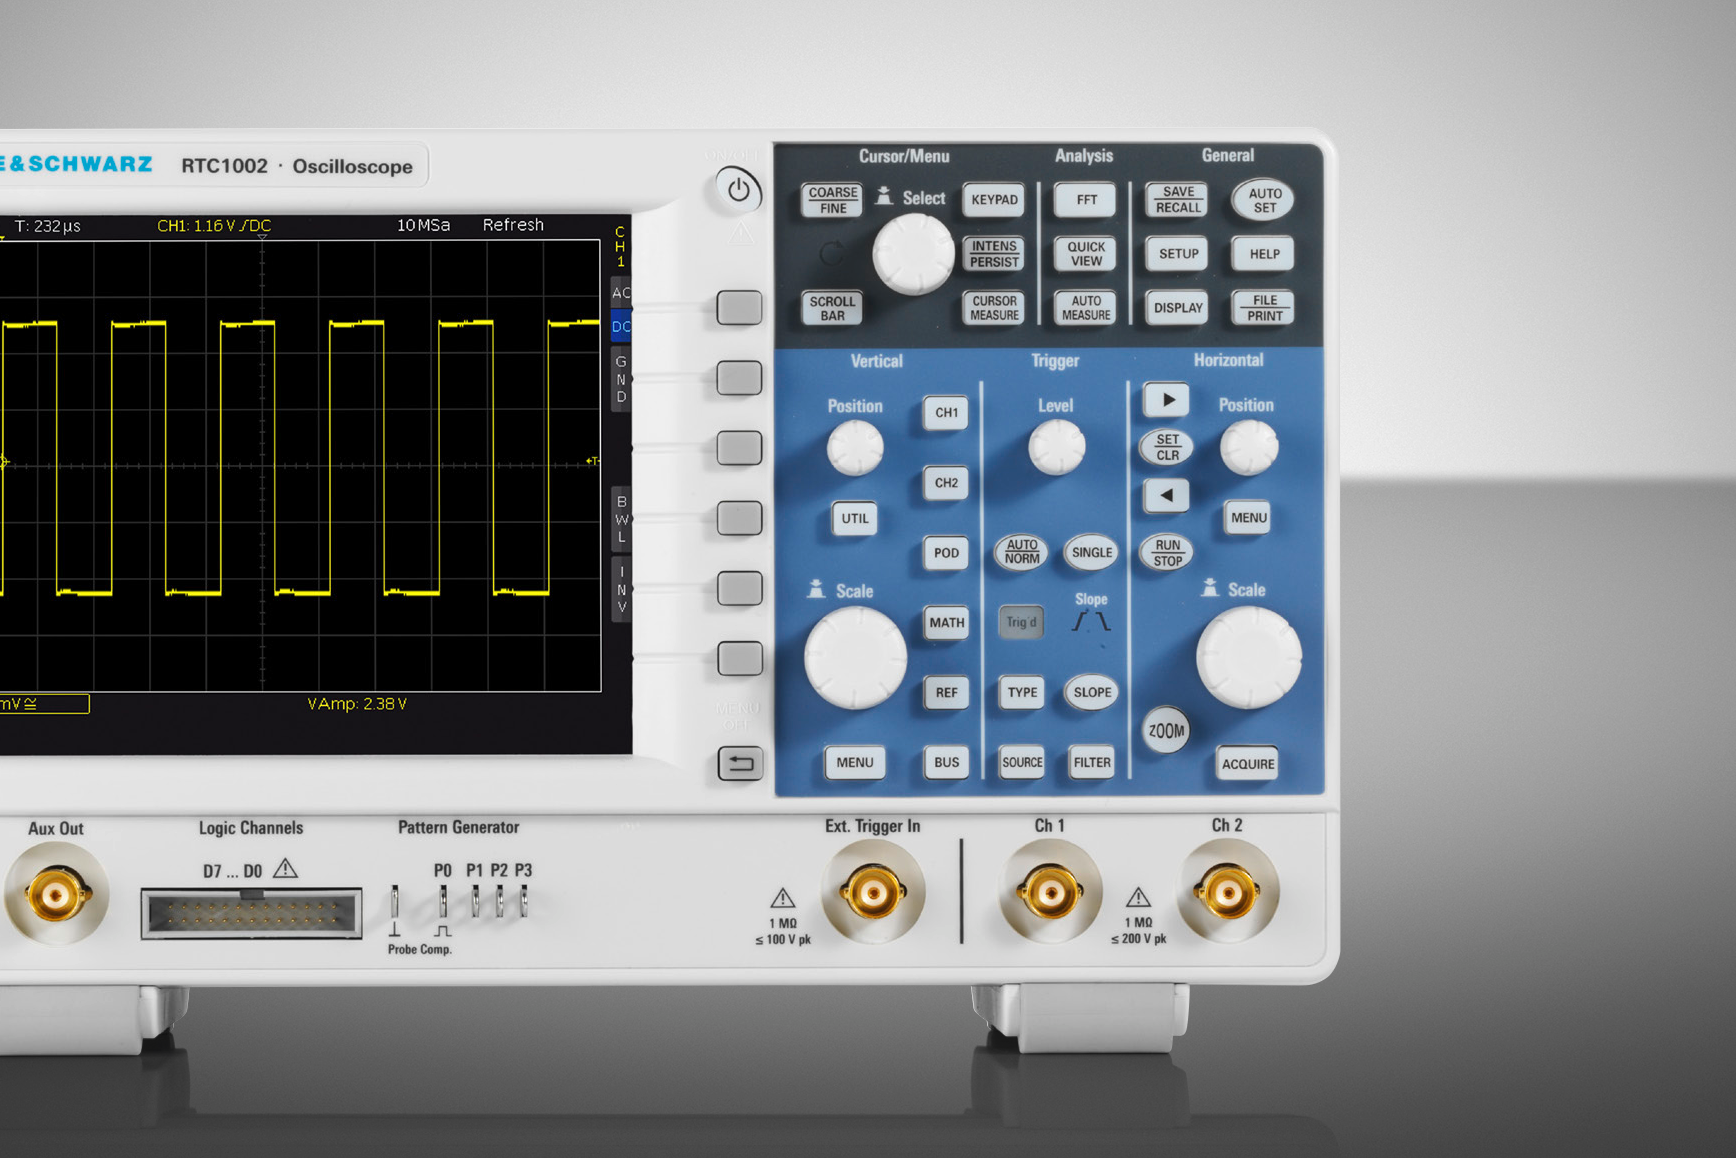
\includegraphics[width=0.50\linewidth, height=5.5cm]{fig_osciloscopio}
    \caption{Osciloscopio digital Rohde \& Schwarz HMO1202 / RTC1002 de \qty{200}{\mega\hertz} y \qty{2}{\giga\sample\per\second}.}
    \label{fig:mat_osciloscopio}
\end{figure}

\begin{figure}[H]
    \centering
    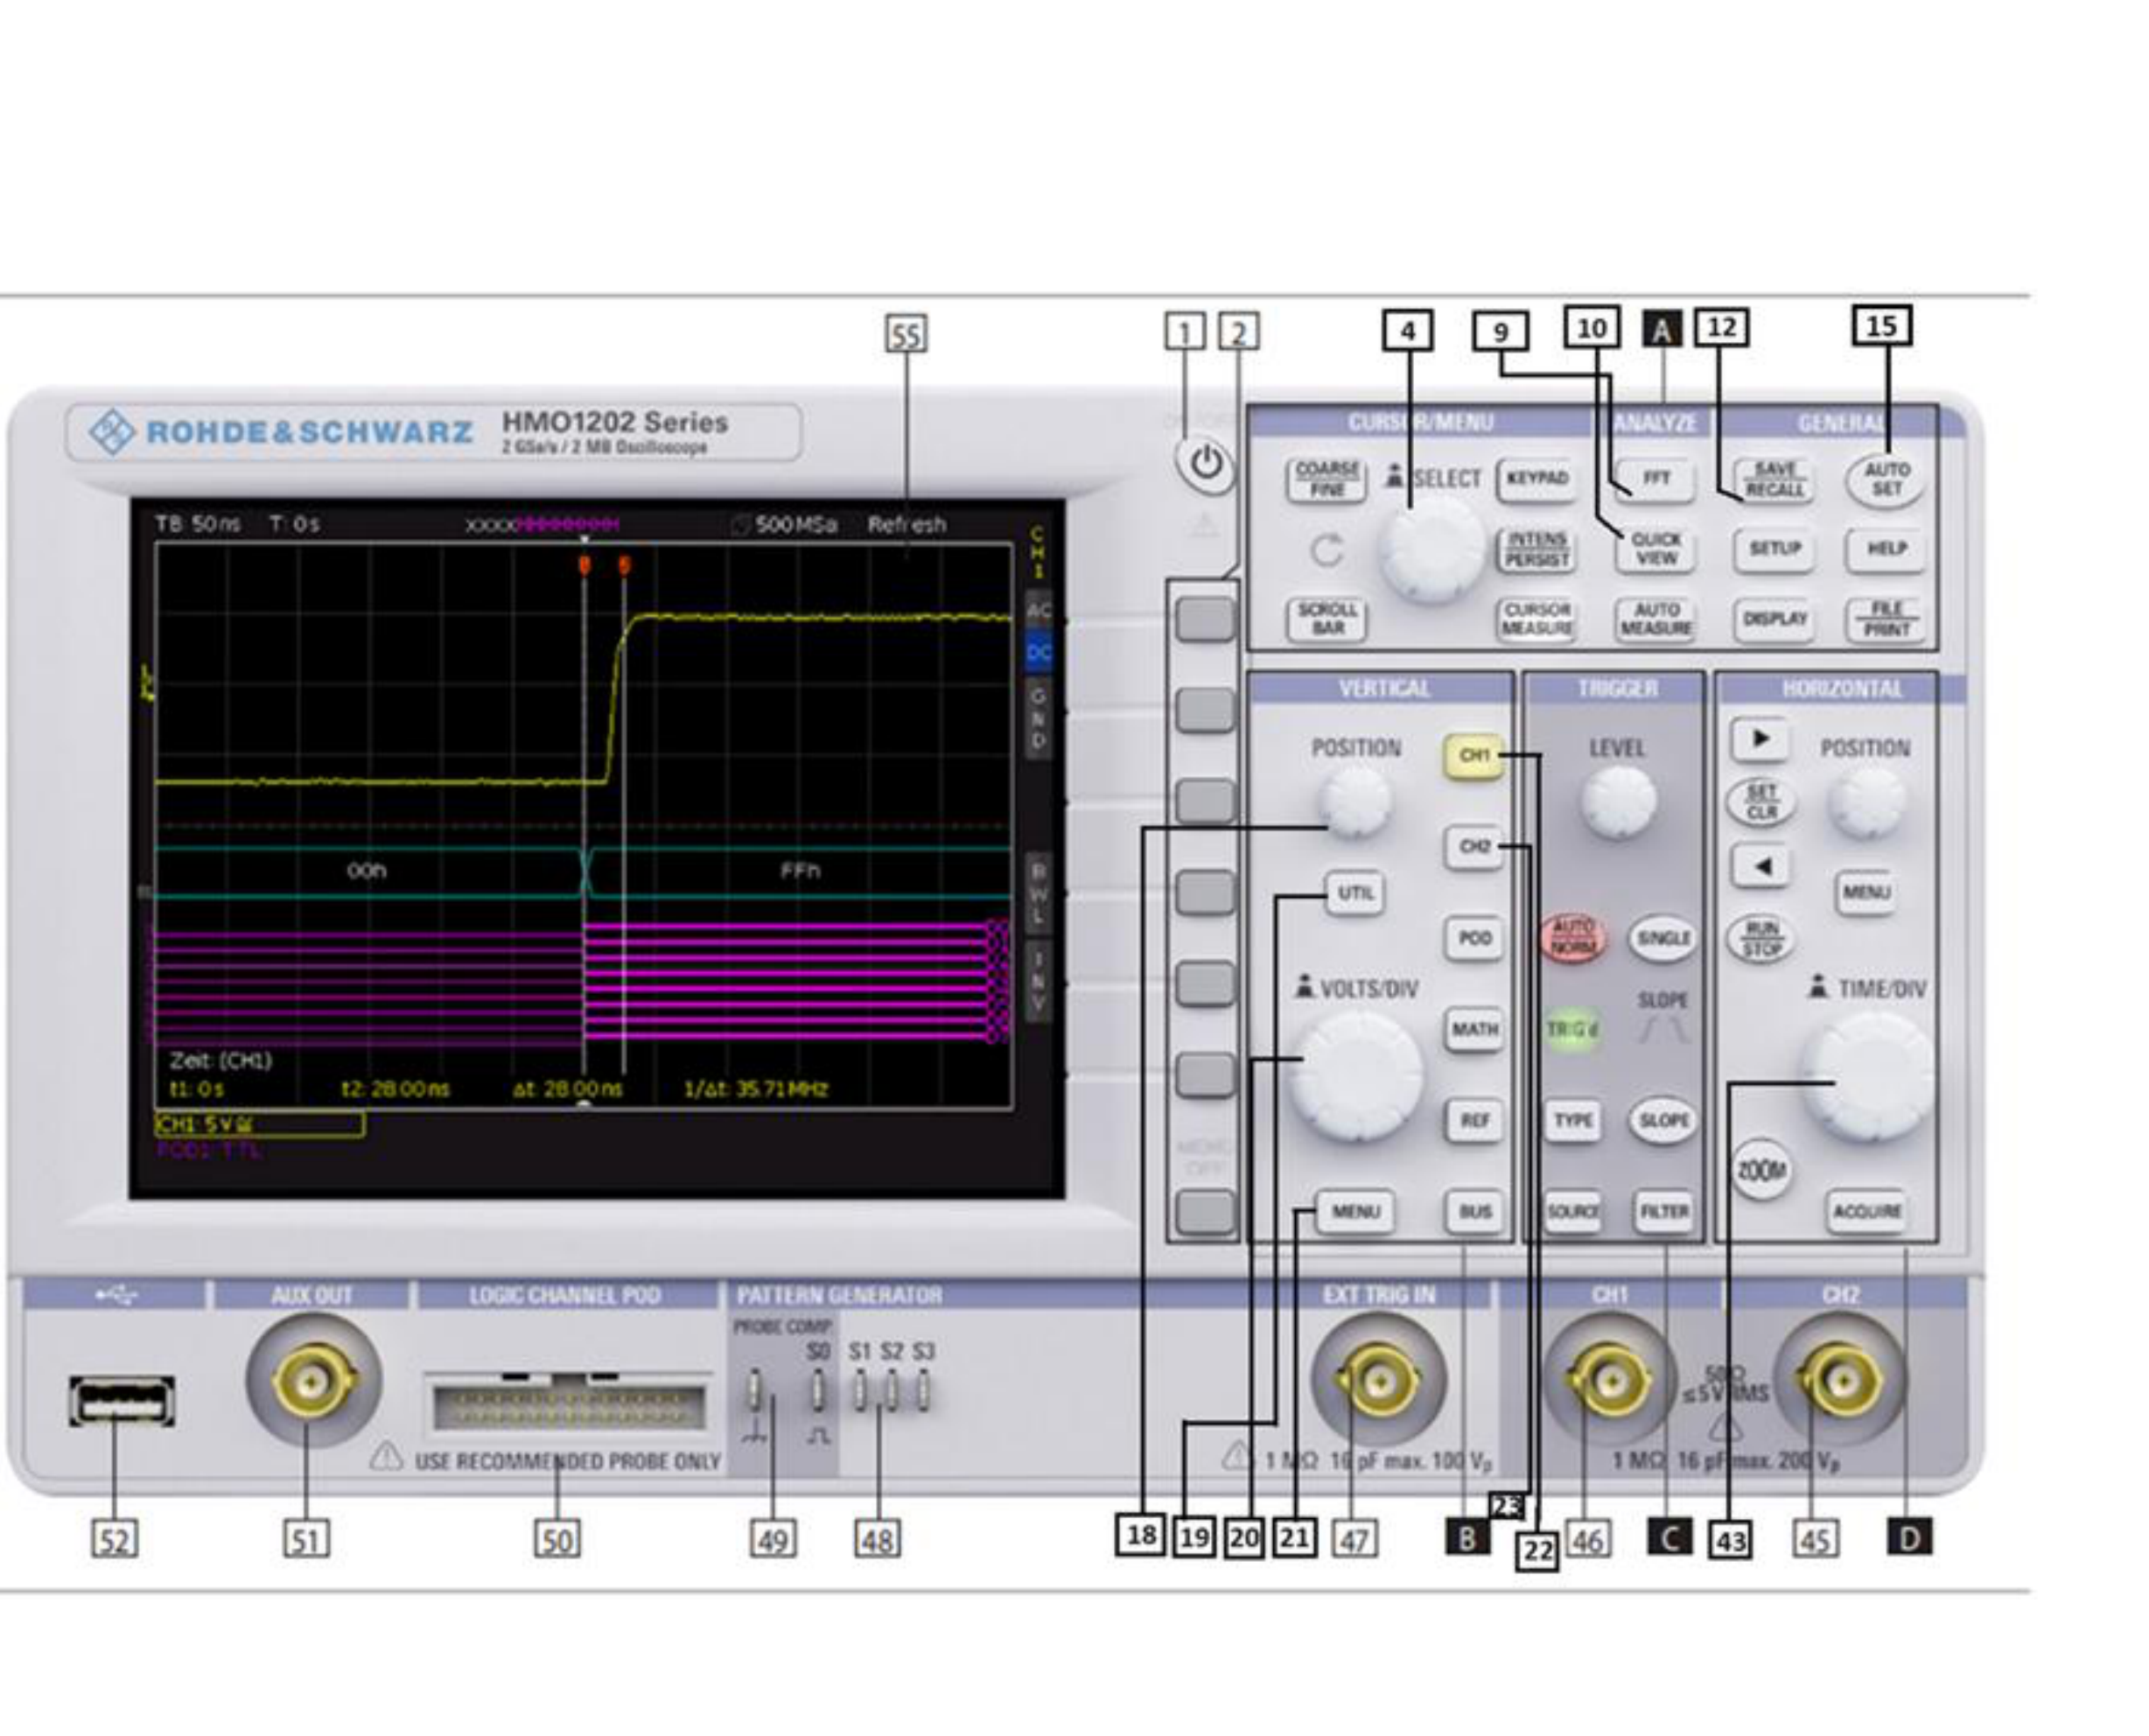
\includegraphics[width=0.50\linewidth, height=5.5cm]{fig_osciloscopio_guia}
    \caption{Panel frontal y disposición de controles del osciloscopio digital de laboratorio~\cite{rs_rtc1000_specs}.}
    \label{fig:mat_panel}
\end{figure}

\begin{itemize}
    \item \textbf{Generador de Funciones Arbitrarias OWON AG 051F (Serie AG-S):}
    \begin{itemize}
        \item Rango de frecuencia: \qty{1}{\micro\hertz} a \qty{5}{\mega\hertz} con resolución de \qty{1}{\micro\hertz} ($\pm\qty{1}{\ppm}$).
        \item Conversión DAC: Resolución vertical de $14\text{ bits}$ y tasa de muestreo de \qty{125}{\mega\sample\per\second}.
        \item Rango de amplitud: \qty{20}{\millivoltpp} a \qty{20}{\voltpp} en alta impedancia ($\text{High-Z}$).
        \item Formas de onda: Senoidal, triangular/rampa, cuadrada, pulso y ruido blanco.
    \end{itemize}
\end{itemize}

\begin{figure}[H]
    \centering
    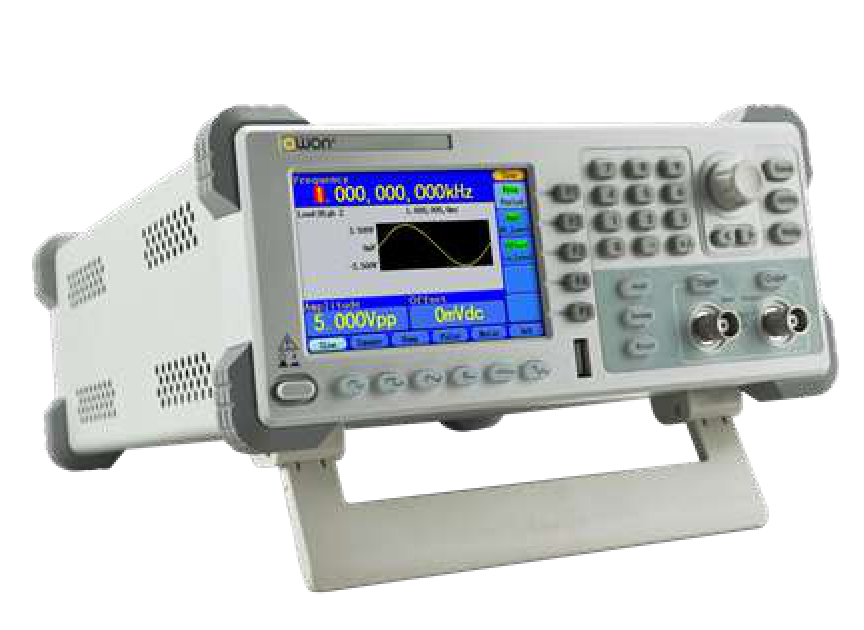
\includegraphics[width=0.50\linewidth, height=5.5cm]{fig_generador}
    \caption{Generador de funciones arbitrarias OWON AG 051F de \qty{5}{\mega\hertz} por síntesis digital directa (DDS).}
    \label{fig:mat_generador}
\end{figure}

\begin{itemize}
    \item \textbf{Multímetro Digital Portátil True-RMS:}
    \begin{itemize}
        \item Escala de tensión continua ($\text{DCV}$): Resolución de \qty{0,001}{\volt}, especificación de fabricante $\pm(\qty{0,5}{\percent} + 2\text{ dígitos})$, resultando en $\delta V_{\text{DC}} = \qty{\pm 0,001}{\volt}$ en el rango de medida evaluado.
        \item Escala de tensión alterna ($\text{ACV}$ True-RMS): Resolución de \qty{0,01}{\volt}, especificación de fabricante $\pm(\qty{1,0}{\percent} + 3\text{ dígitos})$, resultando en $\delta V_{\text{AC}} = \qty{\pm 0,01}{\volt}$ para las lecturas de red.
        \item Ancho de banda de respuesta True-RMS en AC: \qty{40}{\hertz} a \qty{1}{\kilo\hertz}.
    \end{itemize}
\end{itemize}

\begin{figure}[H]
    \centering
    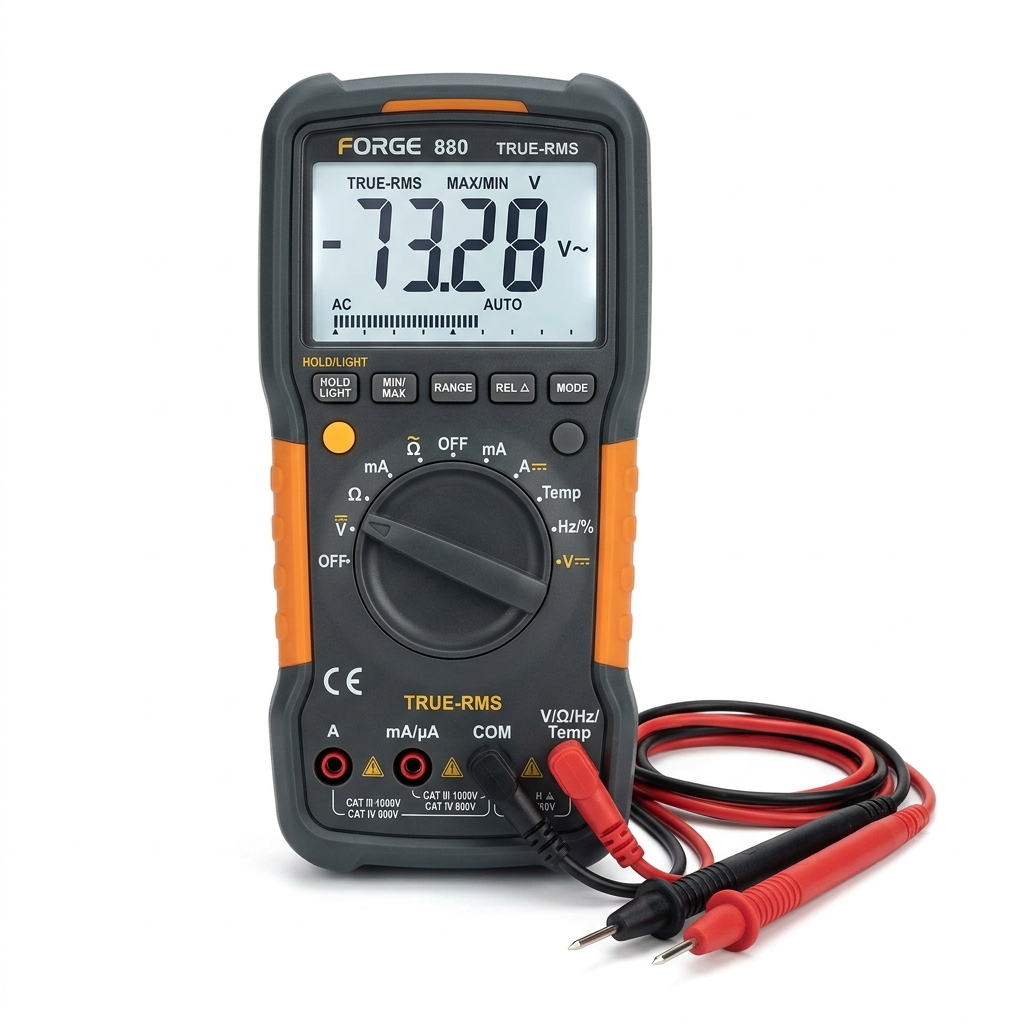
\includegraphics[width=0.50\linewidth, height=5.5cm]{fig_multimetro}
    \caption{Multímetro digital industrial True-RMS utilizado como instrumento patrón de calibración en tensión continua y alterna.}
    \label{fig:mat_multimetro}
\end{figure}

\begin{itemize}
    \item \textbf{Transformador Reductor AC ($220\,\unit{\volt} \to 6\,\unit{\volt}$):}
    \begin{itemize}
        \item Tensión de primario: \qty{220}{\voltrms} a \qty{60}{\hertz} (red eléctrica comercial).
        \item Tensión secundaria nominal: \qty{6,0}{\voltrms} a \qty{60}{\hertz}.
        \item Aislamiento galvánico entre devanados con núcleo de hierro-silicio laminado.
    \end{itemize}
\end{itemize}

\begin{figure}[H]
    \centering
    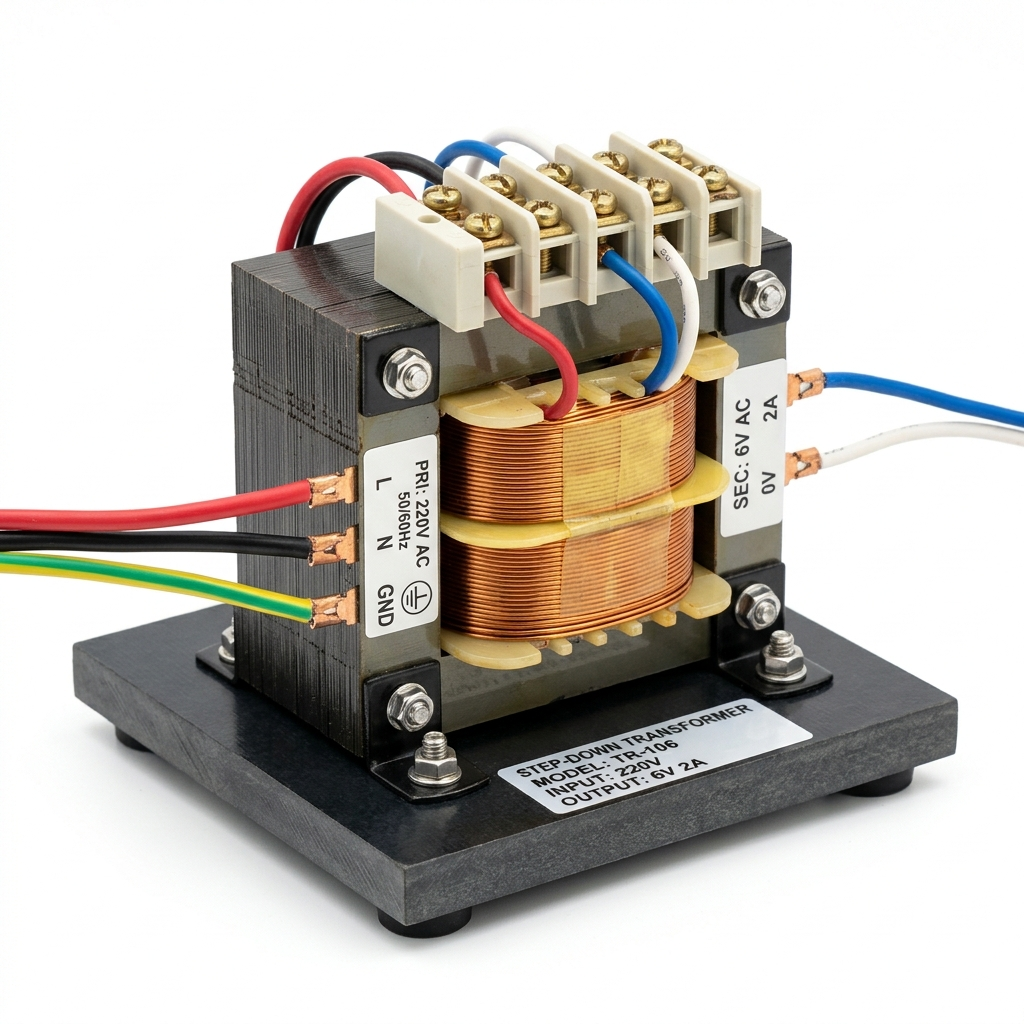
\includegraphics[width=0.50\linewidth, height=5.5cm]{fig_transformador}
    \caption{Transformador reductor monofásico de núcleo laminado para generación de tensión senoidal de \qty{6}{\volt} a \qty{60}{\hertz}.}
    \label{fig:mat_transformador}
\end{figure}

\begin{itemize}
    \item \textbf{Fuente de Tensión Continua Regulada Multisalida:}
    \begin{itemize}
        \item Salidas fijas conmutables: \qty{2,5}{\volt}, \qty{4,5}{\volt}, \qty{7,5}{\volt} y \qty{10,5}{\volt} con rizado $\Delta V_{\text{ripple}} < \qty{8}{\milli\volt}$.
        \item Regulación de línea y carga: $\pm\qty{0,5}{\percent}$ con protección contra cortocircuito.
        \item Conectores de salida de seguridad tipo banana hembra de \qty{4}{\milli\meter}.
    \end{itemize}
\end{itemize}

\begin{figure}[H]
    \centering
    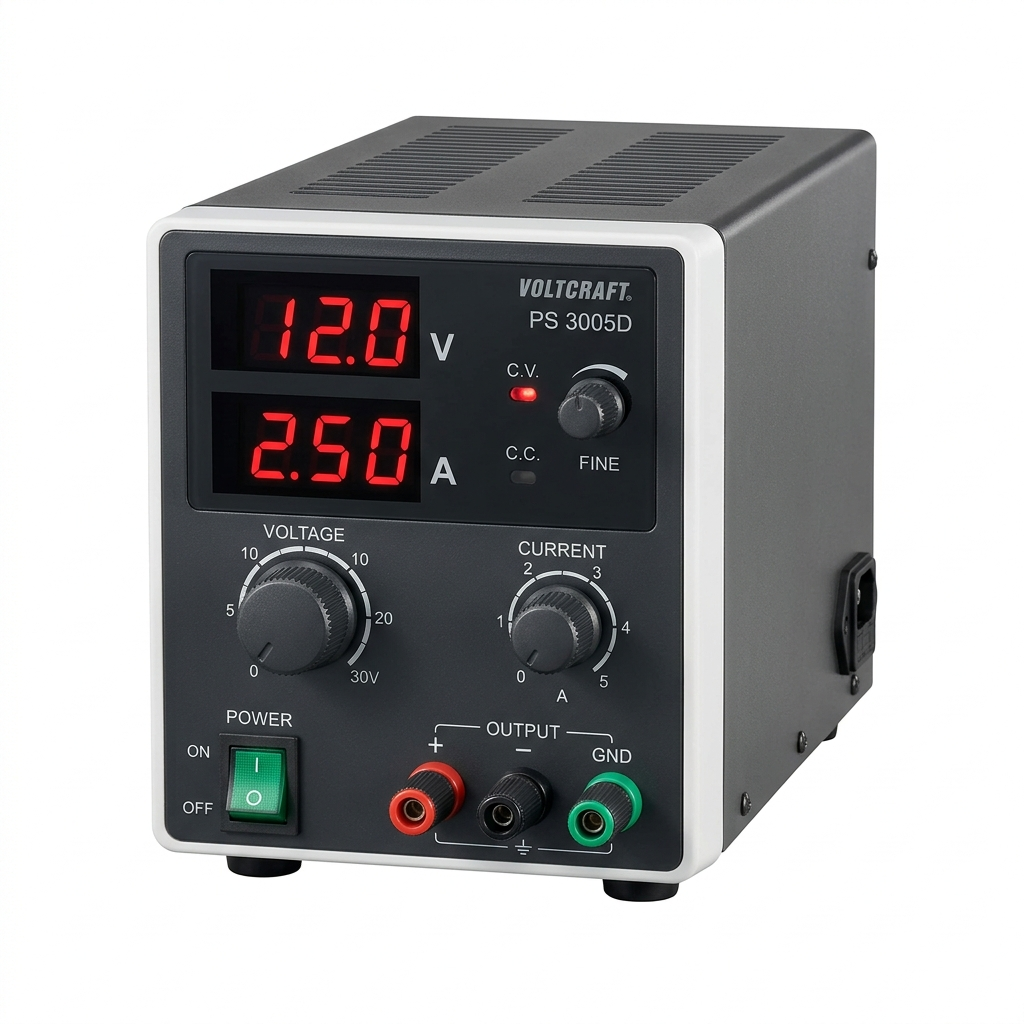
\includegraphics[width=0.50\linewidth, height=5.5cm]{fig_fuente_dc}
    \caption{Fuente regulada lineal de tensión continua de banco con salidas fijas escalonadas.}
    \label{fig:mat_fuente_dc}
\end{figure}

\begin{itemize}
    \item \textbf{Pila Cilíndrica Alcalina (AA):}
    \begin{itemize}
        \item Tensión nominal electroquímica de celda: \qty{1,50}{\volt} (sistema dióxido de manganeso-zinc $\text{Zn}/\text{MnO}_2$).
        \item Capacidad energética nominal: $\sim\qty{2500}{\milli\ampere\hour}$.
        \item Resistencia interna reducida ($r_i \approx \qty{0,15}{\ohm}$), ideal como patrón DC libre de componentes de rizado.
    \end{itemize}
\end{itemize}

\begin{figure}[H]
    \centering
    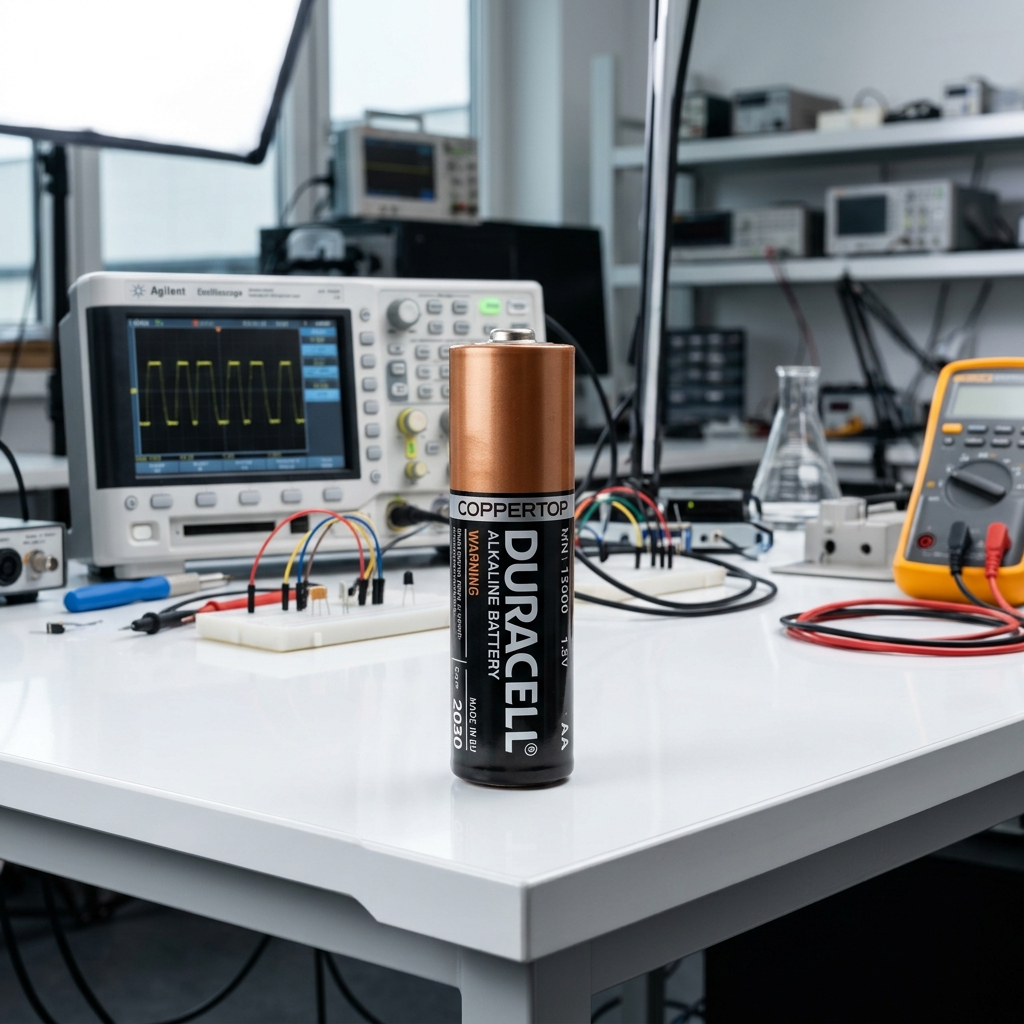
\includegraphics[width=0.50\linewidth, height=5.5cm]{fig_pila_aa}
    \caption{Pila cilíndrica alcalina estándar tipo AA de \qty{1,50}{\volt} utilizada para contraste y calibración DC.}
    \label{fig:mat_pila_aa}
\end{figure}

\begin{itemize}
    \item \textbf{Cables de Conexión Coaxial BNC y Puntas Banana-Cocodrilo:}
    \begin{itemize}
        \item Cables coaxiales blindados de \qty{50}{\ohm} con conectores BNC macho hacia terminales cocodrilo aislados.
        \item Cables de prueba flexibles con conectores banana apilables de \qty{4}{\milli\meter} a pinzas cocodrilo de agarre firme.
        \item Aislamiento dieléctrico de alta rigidez para mediciones seguras de hasta \qty{600}{\voltrms}.
    \end{itemize}
\end{itemize}

\begin{figure}[H]
    \centering
    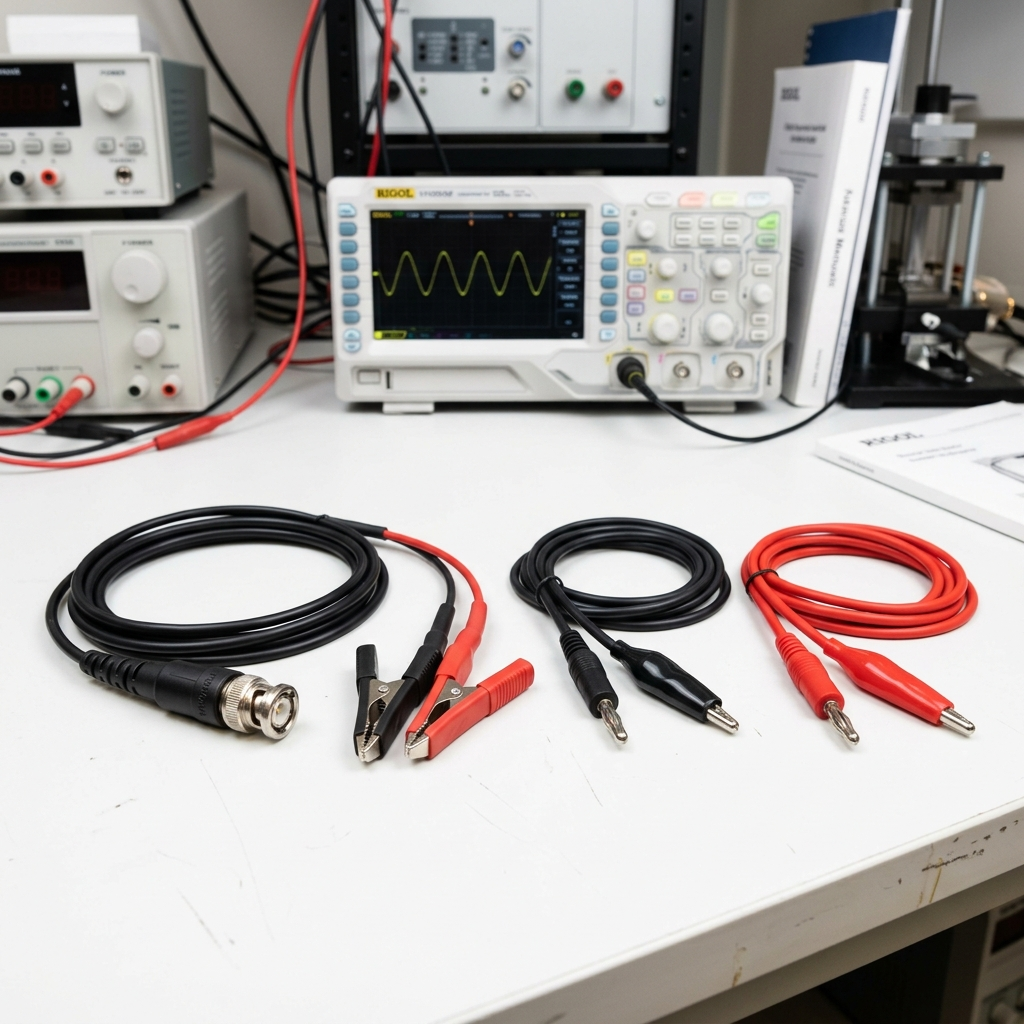
\includegraphics[width=0.50\linewidth, height=5.5cm]{fig_cables_sondas}
    \caption{Cables de conexión coaxial BNC y líneas de prueba con conectores banana y pinzas cocodrilo.}
    \label{fig:mat_cables_sondas}
\end{figure}

\subsection{Tabla Resumen de Especificaciones de los Instrumentos}

En la Tabla~\ref{tab:especificaciones_instrumentos} se sintetizan las especificaciones metrológicas fundamentales, rangos de operación e incertidumbres instrumentales declaradas para todos los equipos utilizados en la práctica.

\begin{table}[H]
    \centering
    \caption{Especificaciones metrológicas de los equipos e instrumentos empleados.}
    \label{tab:especificaciones_instrumentos}
    \resizebox{\linewidth}{!}{%
    \begin{tabular}{@{}llll@{}}
        \toprule
        \textbf{Instrumento} & \textbf{Modelo / Marca} & \textbf{Rango de Medida} & \textbf{Incertidumbre Instrumental ($\delta x$)} \\
        \midrule
        Osciloscopio Digital & R\&S HMO1202 / RTC1002 & $\qty{0}{\mega\hertz}\text{ a }\qty{200}{\mega\hertz},\; \qty{1}{\milli\volt\per\division}\text{ a }\qty{10}{\volt\per\division}$ & $\delta N_{\text{div}} = \pm 0{,}1\,\text{div},\; \delta f/f = \pm\qty{0,05}{\percent}$ \\
        Generador de Señales & OWON AG 051F & $\qty{1}{\micro\hertz}\text{ a }\qty{5}{\mega\hertz},\; \qtyrange{0,02}{20}{\voltpp}$ & $\delta f/f = \pm\qty{1}{\ppm},\; \delta V_p = \pm\qty{0,05}{\volt}$ \\
        Multímetro Digital   & Industrial True-RMS    & $\qtyrange{0}{600}{\volt}\; (\text{DC/AC})$ & $\pm(\qty{0,5}{\percent} + 2\,\text{dgt}) \to \pm\qty{0,001}{\volt},\; \pm(\qty{1,0}{\percent} + 3\,\text{dgt}) \to \pm\qty{0,01}{\volt}$ \\
        Transformador AC     & Reductor Monofásico    & $\qty{220}{\volt} \to \qty{6}{\volt},\; \qty{60}{\hertz}$ & $\delta f_{\text{red}} = \pm\qty{0,05}{\hertz}$ \\
        Fuente Regulada DC   & Multisalida de Banco   & $\qtyrange{2,5}{10,5}{\volt}$ & $\delta V_{\text{mult}} = \pm\qty{0,001}{\volt}$ \\
        Pila Alcalina        & Cilíndrica AA          & \qty{1,50}{\volt} nominal & $\delta V_{\text{mult}} = \pm\qty{0,001}{\volt}$ \\
        Cables y Sondas      & Coaxial BNC / Banana   & $\qty{50}{\ohm},\; \qty{600}{\voltrms}\text{ máx.}$ & Atenuación despreciable en baja frecuencia \\
        \bottomrule
    \end{tabular}%
    }
\end{table}